\chapter{Theoretical Shenanigans}

\begin{theorem}[Couto et al.\cite{couto2011exact}]
When given a polygon $P$ and a guard set $G$, a subset $G_{sub}$ of $G$ fully covers $P$ if and only if it covers all witnesses in the shadow witness set $W$ of $G$.
\end{theorem}
\begin{proof}
The necessity condition follows trivially from $W\in P$. As for the sufficiency condition, consider the largest area $R$ that is not covered by $G_{sub}$. Because of the atomicity of AVPs, $R$ must consist of one or more AVPs. Now consider the AVP $f$ with minimal guard subset $G_{f}$ in $R$. We show that $f$ must be a shadow AVP, a contradiction. If $f = R$, then $f$ trivially must be a shadow AVP. Otherwise, consider the neighbors of $f$. For all neighbors in $R$, $G_{f}$ can not contain their guard subset as $G_{f}$ is minimal in R. As for the neighbors not in $R$, if there exists a neighbor of which the guard subset is contained in $G_{f}$, then $f$ must be covered by one of the guards in that subset and can not be part of $R$. Otherwise, $G_{f}$ does not contain any of its neighbors' guard subsets and thus is a shadow AVP.
\end{proof}

\begin{theorem}
When given a polygon $P$ and a guard set $G$, the guard subsets of a light polygon form a clique in the 2-link-visibility graph $G_{vis}$ of $G$, and the cliques of all light polygons cover all edges of the graph.
\end{theorem}
\begin{proof}
The guard subset of a light polygon is formed by all the guards whose visibility polygons intersect in it, thus trivially forming a clique in $G_{vis}$. Assuming that for $g,g'\in G$ there exists an edge $(g, g')$ in $G_{vis}$ that is not covered by those cliques, then there exists an AVP $f$ that is not light and contains $g$ and $g'$ in its guard subset $G_{sub}$. As $f$ is not light there exists a neighboring AVP $f'$ whose guard subset contains $G_{sub}$. One can continue this argument with $f'$, but as the number of AVPs is finite, we will eventually reach an AVP $f^{*}$ of which the guard subset is not contained in its neighbors. Thus, $f^{*}$ is a light AVP and contains $g$ and $g'$, a contradiction.
\end{proof}

\begin{figure}[htbp]
\centering
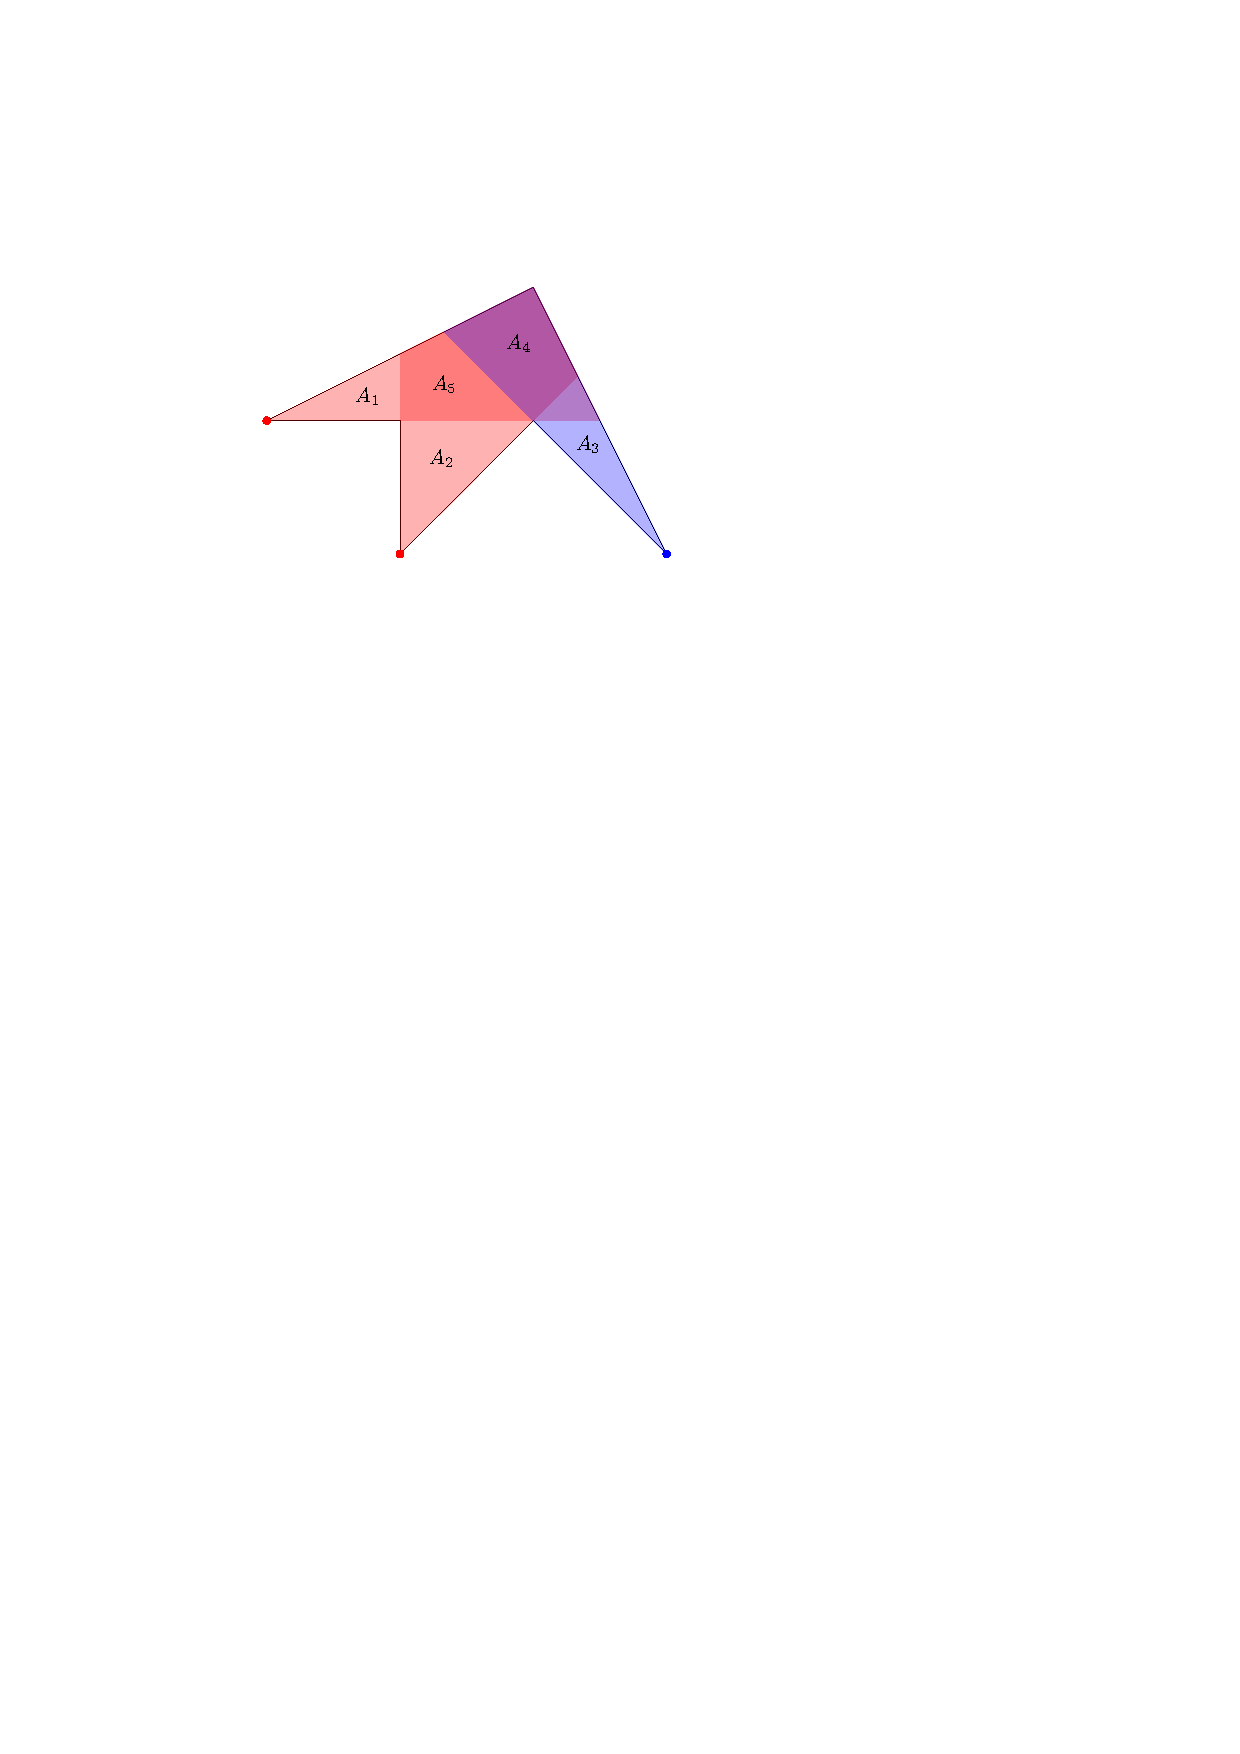
\includegraphics[scale=1.3]{Thesis/figures/conflict-free_witnesses.pdf}
\caption{Illustration for the proof of \cref{thm:light_covers}.}
\label{fig:light_covers}
\end{figure}

\begin{theorem}\label{thm:light_covers}
For a polygon $P$ and a guard set $G$, neither conflict-freeness of all shadow witnesses nor all light witnesses guarantees conflict-freeness within all AVPs.
\end{theorem}
\begin{proof}
To prove this theorem, we present a simple example in \cref{fig:light_covers}. In the figure $A_{1}$, $A_{2}$ and $A_{3}$ are shadow AVPs and $A_{4}$ is a light AVP. Each of them is covered by a guard of unique color. On the other hand, $A_{5}$ is neither shadow nor light and is covered by two guards of the same color, thus is not conflict-free.
\end{proof}

\chapter{Chromatic Art Gallery Problem Formulations}

\section{MIP Formulation}

\section{SAT Formulation}

\section{CPSAT Formulation}

\chapter{Conflict-free Chromatic Art Gallery Problem Formulations}

\section{MIP Formulation}

\section{SAT Formulation}

\section{CPSAT Formulation}

\chapter{Implementation Details}

\section{Instance Processing}

\section{Initial Upper Bound}

\section{Clique Edge Covers}

\section{Lazy Constraints}